
\newcommand{\paramI}[1]{\text{-}\ensuremath{#1}}
\newcommand{\param}[1]{\text{\--\--}\ensuremath{#1}}

\chapter{TRAVeLer - Template RnA Visualization}

Traveler je konzolová aplikacia programovaná v C++ a je určený pre operačné systemý UNIX-ového typu.
Vyvýjaný a testovaný bol na Linux-e a FreeBSD. Podpora ostatných systémov nieje zaručená.

\section{Inštalácia}

Požadované programové vybavenie je:
\begin{itemize}
  \item gcc verzie aspoň 4.9.2
\end{itemize}

Pri testovaní boli zaznamenané problémy s regulárnymi výrazmi, ktoré nám pomáhajú pri načítavaní
vstupných súborov. Problém bol pri verzií gcc 4.7.2, ktorá plne nepodporovala potrebné výrazy.

Traveler prelozžíme zo zdrojových kódov postupnosťou príkazov z koreňového adresára:
\begin{itemize}
  \item cd src/
  \item make build
    \\
    Následne spustiteľný súbor je $src/build/traveler$.
\end{itemize}

\section{Argumenty programu}

Ak predpokladáme, že program leží na $PATH$, spúšťame ho nasledovne:

\begin{code}[frame=none]
traveler [-h|--help]
traveler [OPTIONS] <TREES>

OPTIONS:
  [-a|--all [--overlaps] [--colored] <FILE_OUT>]
  [-t|--ted <FILE_MAPPING_OUT>]
  [-d|--draw [--overlaps] [--colored] <FILE_MAPPING_IN> <FILE_OUT>]
  [--debug]

TREES:
  <-mt|--match-tree> FILE_FASTA
  <-tt|--template-tree> [--type DOCUMENT_TYPE] DOCUMENT FILE_FASTA
\end{code}

Stručnú nápovedu k programu dostaneme štandardným \paramI{h} alebo \param{help} argumentom.

Prepínačmi \param{ted} a \param{draw} vieme oddeliť fázu počítania vzdialenosti pomocou TEDu a nasledného kreslenia.

Prepínač \param{overlaps} po nakreslení obrázku v ňom vyznačí všetky miesta prekryvov, ak nejaké vznikli.
Zároveň ich počet vypíše do samostatného súboru. Následne rýchlejšie dokážeme identifikovať molekuly, ktoré
potrebujú zvýšenú pozornosť.

Prepínač \param{colored} aktivuje farebné zvýrazňovanie zmien v štruktúre stromu oproti šablone.
Používame nasledovné kódovanie farbami:

\begin{tabular}{@{$\bullet$ }ll}
  $Cervena$ & vložené bázy
  \\
  $Zelena$  & editované bázy
  \\
  $Modra$   & bázy ktoré sme potrebovali presunúť
  \\
  $Hneda$   & podstromy prekreslených multibranch loop
\end{tabular}
\begin{figure}
  XYZ
\caption{Farebné vyznačovanie operácií v obrázku}
\label{tab:traveler_colors}
\end{figure}
\\

Farbami zvýrazňujeme zmeny v strome, to znamená, že ak sa bázový pár zmení v jednej báze,
cely bude označený ako editovaný.

Modrou označujeme časti, ktoré sme z nejakého dôvodu potrebovali presunúť a prekresliť. Typickým príkladom
je prekreslenie loopy po vložení/zmazaní nejakej bázy. Vtedy sme vložili napríklad 1 bázu ale potrebovali
presunúť ďalších 10 ktoré už v loop boli.
% TODO príklad

Hnedou farbou označujeme celé podstromy multibranch loopy, ktorú sme museli prekresliť.
V týchto prípadoch vznikajú často veľké prekryvy a týmto ich odlišujeme od ostatných, nečakanýh.

Prepínač \param{match-tree} nám určuje RNA molekulu ktorú ideme vizualizovať, \param{template-tree}
šablónu. Strom vizualizovanej molekuly sa načítava iba z fasta súboru, kdežto pri šablónovej molekule
potrebujeme aj jej obrázok. Viac informácii ohľadom parametra \param{type} nájdete v kapitole \nameref{kap:rozšírenie}.

\subsection{Formát fasta súboru}

Ako formát súborov kodujúcich stromy používame trochu upravený fasta formát.

Súbor na prvom riadku obsahuje názov molekuly hned za znakom $>$ az po prvú medzeru.
Na ďalších riadkoch obsahuje znaky sekvencie RNA a znaky kódujúce sekundárnu štruktúru.
Je zvykom, ze riadky su siroke najviac 80 znakov.

Fasta súbor pre šablonovú molekulu RNA potrebuje iba názov a zatvorkovanie, pre
vizualizovanú molekulu aj sekvenciu. Je to dané tým, že sekvenciu si vieme vybrať z obrázka šablony.

\section{Príklad vstupu}

Teraz uvedieme príklad vstupu pre malú podjednotku ribozomálnej RNA myši, konkrétne príklad
fasta súboru \ref{obr:mouse_fasta}, podporovaného formátu post script súboru \ref{obr:mouse_ps_text}
a následne aj obrázok vizualizácie v post script súbore \ref{obr:mouse_ps}.

\begin{pozn}
  Podporujeme iba jeden formát PostScript súborov - ten používa databáza CRW publikovaná \citet{CRW}.
  Ďalšie rozšírenia podpory iných formátov rozoberáme v kapitole \nameref{kap:rozšírenie}.
\end{pozn}

\begin{figure}[H]
\begin{code}[fontsize=\scriptsize, frame=none, samepage=true]
>mouse
UACCUGGUUGAUCCUGCCAGUAGCAUAUGCUUGUCUCAAAGAUUAAGCCAUGCAUGUCUAAGUACGCACGGCCGGUACAG
UGAAACUGCGAAUGGCUCAUUAAAUCAGUUAUGGUUCCUUUGGUCGCUCGCUCCUCUCCUACUUGGAUAACUGUGGUAAU
UCUAGAGCUAAUACAUGCCGACGGGCGCUGACCCCCCUUCCCGGGGGGGGAUGCGUGCAUUUAUCAGAUCAAAACCAACC
CGGUGAGCUCCCUCCCGGCUCCGGCCGGGGGUCGGGCGCCGGCGGCUUGGUGACUCUAGAUAACCUCGGGCCGAUCGCAC
GCCCCCCGUGGCGGCGACGACCCAUUCGAACGUCUGCCCUAUCAACUUUCGAUGGUAGUCGCCGUGCCUACCAUGGUGAC
CACGGGUGACGGGGAAUCAGGGUUCGAUUCCGGAGAGGGAGCCUGAGAAACGGCUACCACAUCCAAGGAAGGCAGCAGGC
GCGCAAAUUACCCACUCCCGACCCGGGGAGGUAGUGACGAAAAAUAACAAUACAGGACUCUUUCGAGGCCCUGUAAUUGG
AAUGAGUCCACUUUAAAUCCUUUAACGAGGAUCCAUUGGAGGGCAAGUCUGGUGCCAGCAGCCGCGGUAAUUCCAGCUCC
AAUAGCGUAUAUUAAAGUUGCUGCAGUUAAAAAGCUCGUAGUUGGAUCUUGGGAGCGGGCGGGCGGUCCGCCGCGAGGCG
AGUCACCGCCCGUCCCCGCCCCUUGCCUCUCGGCGCCCCCUCGAUGCUCUUAGCUGAGUGUCCCGCGGGGCCCGAAGCGU
UUACUUUGAAAAAAUUAGAGUGUUCAAAGCAGGCCCGAGCCGCCUGGAUACCGCAGCUAGGAAUAAUGGAAUAGGACCGC
GGUUCUAUUUUGUUGGUUUUCGGAACUGAGGCCAUGAUUAAGAGGGACGGCCGGGGGCAUUCGUAUUGCGCCGCUAGAGG
UGAAAUUCUUGGACCGGCGCAAGACGGACCAGAGCGAAAGCAUUUGCCAAGAAUGUUUUCAUUAAUCAAGAACGAAAGUC
GGAGGUUCGAAGACGAUCAGAUACCGUCGUAGUUCCGACCAUAAACGAUGCCGACUGGCGAUGCGGCGGCGUUAUUCCCA
UGACCCGCCGGGCAGCUUCCGGGAAACCAAAGUCUUUGGGUUCCGGGGGGAGUAUGGUUGCAAAGCUGAAACUUAAAGGA
AUUGACGGAAGGGCACCACCAGGAGUGGGCCUGCGGCUUAAUUUGACUCAACACGGGAAACCUCACCCGGCCCGGACACG
GACAGGAUUGACAGAUUGAUAGCUCUUUCUCGAUUCCGUGGGUGGUGGUGCAUGGCCGUUCUUAGUUGGUGGAGCGAUUU
GUCUGGUUAAUUCCGAUAACGAACGAGACUCUGGCAUGCUAACUAGUUACGCGACCCCCGAGCGGUCGGCGUCCCCCAAC
UUCUUAGAGGGACAAGUGGCGUUCAGCCACCCGAGAUUGAGCAAUAACAGGUCUGUGAUGCCCUUAGAUGUCCGGGGCUG
CACGCGCGCUACACUGACUGGCUCAGCGUGUGCCUACCCUGCGCCGGCAGGCGCGGGUAACCCGUUGAACCCCAUUCGUG
AUGGGGAUCGGGGAUUGCAAUUAUUCCCCAUGAACGAGGAAUUCCCAGUAAGUGCGGGUCAUAAGCUUGCGUUGAUUAAG
UCCCUGCCCUUUGUACACACCGCCCGUCGCUACUACCGAUUGGAUGGUUUAGUGAGGCCCUCGGAUCGGCCCCGCCGGGG
UCGGCCCACGGCCCUGGCGGAGCGCUGAGAAGACGGUCGAACUUGACUAUCUAGAGGAAGUAAAAGUCGUAACAAGGUUU
CCGUAGGUGAACCUGCGGAAGGAUCAUUA
...(((((.......))))).((((((((((.(((((((((.....(((.(((..((...(((....((..........)
)...)))))......(((......((((..((..((....(((..................((((....(((((((....
.))))))).....)))).......((((...((((((......))))))...))))....((((((.......(((((.(
(((...((((.((((((((....))))))))..)))).))))....)))))......))))))...........((((.(
(((......))))))))....)))...))))..))))(((..(.(((....((((((((.......)))))))))))...
..))))...((((((((....))))...))))))).((((((..........)))))).((((....))))...))))))
.).....(.(((...(((((...))))).)))).)).))))))....(((((((((.(((....)))..)))))).))).
.....(((.(((.......)))).)).........((((((.......((((.....((....)).......))))))))
)).))))))))))..........(((.......((((...(((.......(((.(((((((((((((.((((....))))
....))))))))..)))))))).......((((.(((((...(((((((......)))))))....))))))))).....
................................................................................
...........................................(((((((((..(((((((((..((((((((...(((.
.....)))......))))))))..))....(..((....)))))))))).))))).))))...)))...))))....(((
(((...((...((((.........))))...))))))))..........((((((.(((..((((((((.(((((....)
))))))))))))..)))...((....))...)))....))).)))..(((.....((((....))))....)))......
..(((((.(((((((..((..((((((((((((((((....((((........))))........(((((((....((((
(........((((((........))))))......)))))...((.((((..(((((((((...(((((((((....)))
..((((......))))..)))))).....((((.(((.((((..((((....(((..((((....)))).)))....)))
)..)))))))..((((((((.....))))))))....))))...)))).)))...).))))))).....)))))))...)
).))))))).))...(((((((.....(((.......((..((((....))))..)).....))).....)))))))...
...(...((((((((........))))))))...).....))))).....((((((((.......))))))))......)
)...)))))))))).))....((.((.(.((((((((.((.((((((((((((..(((((((((((((((.(((((((((
(((.....))))))))))))...)))))))))))))))..))))))))))))).)))))))))..).))..))....(((
(((((((....))))))))))........
\end{code}
\caption{Príklad fasta súboru}
\label{obr:mouse_fasta}
\end{figure}

\begin{figure}[H]
\begin{code}[fontsize=\scriptsize, frame=none, samepage=true]
%!
/lwline {newpath moveto lineto stroke} def
  ...
434.00 -129.00 422.00 -138.00 lwline
0.00 setlinewidth
446.00 -421.00 446.00 -412.00 lwline
306.00 -283.00 306.00 -273.00 lwline
  ...
(U) 303.30 -273.00 lwstring
(A) 303.30 -265.00 lwstring
(C) 303.30 -257.00 lwstring
(C) 303.50 -248.68 lwstring
(U) 311.24 -246.68 lwstring
(G) 318.99 -244.68 lwstring
  ...
\end{code}
\caption{Príklad podporovaného formátu post script súboru}
\label{obr:mouse_ps_text}
\end{figure}

\begin{figure}
  \makebox[\textwidth]{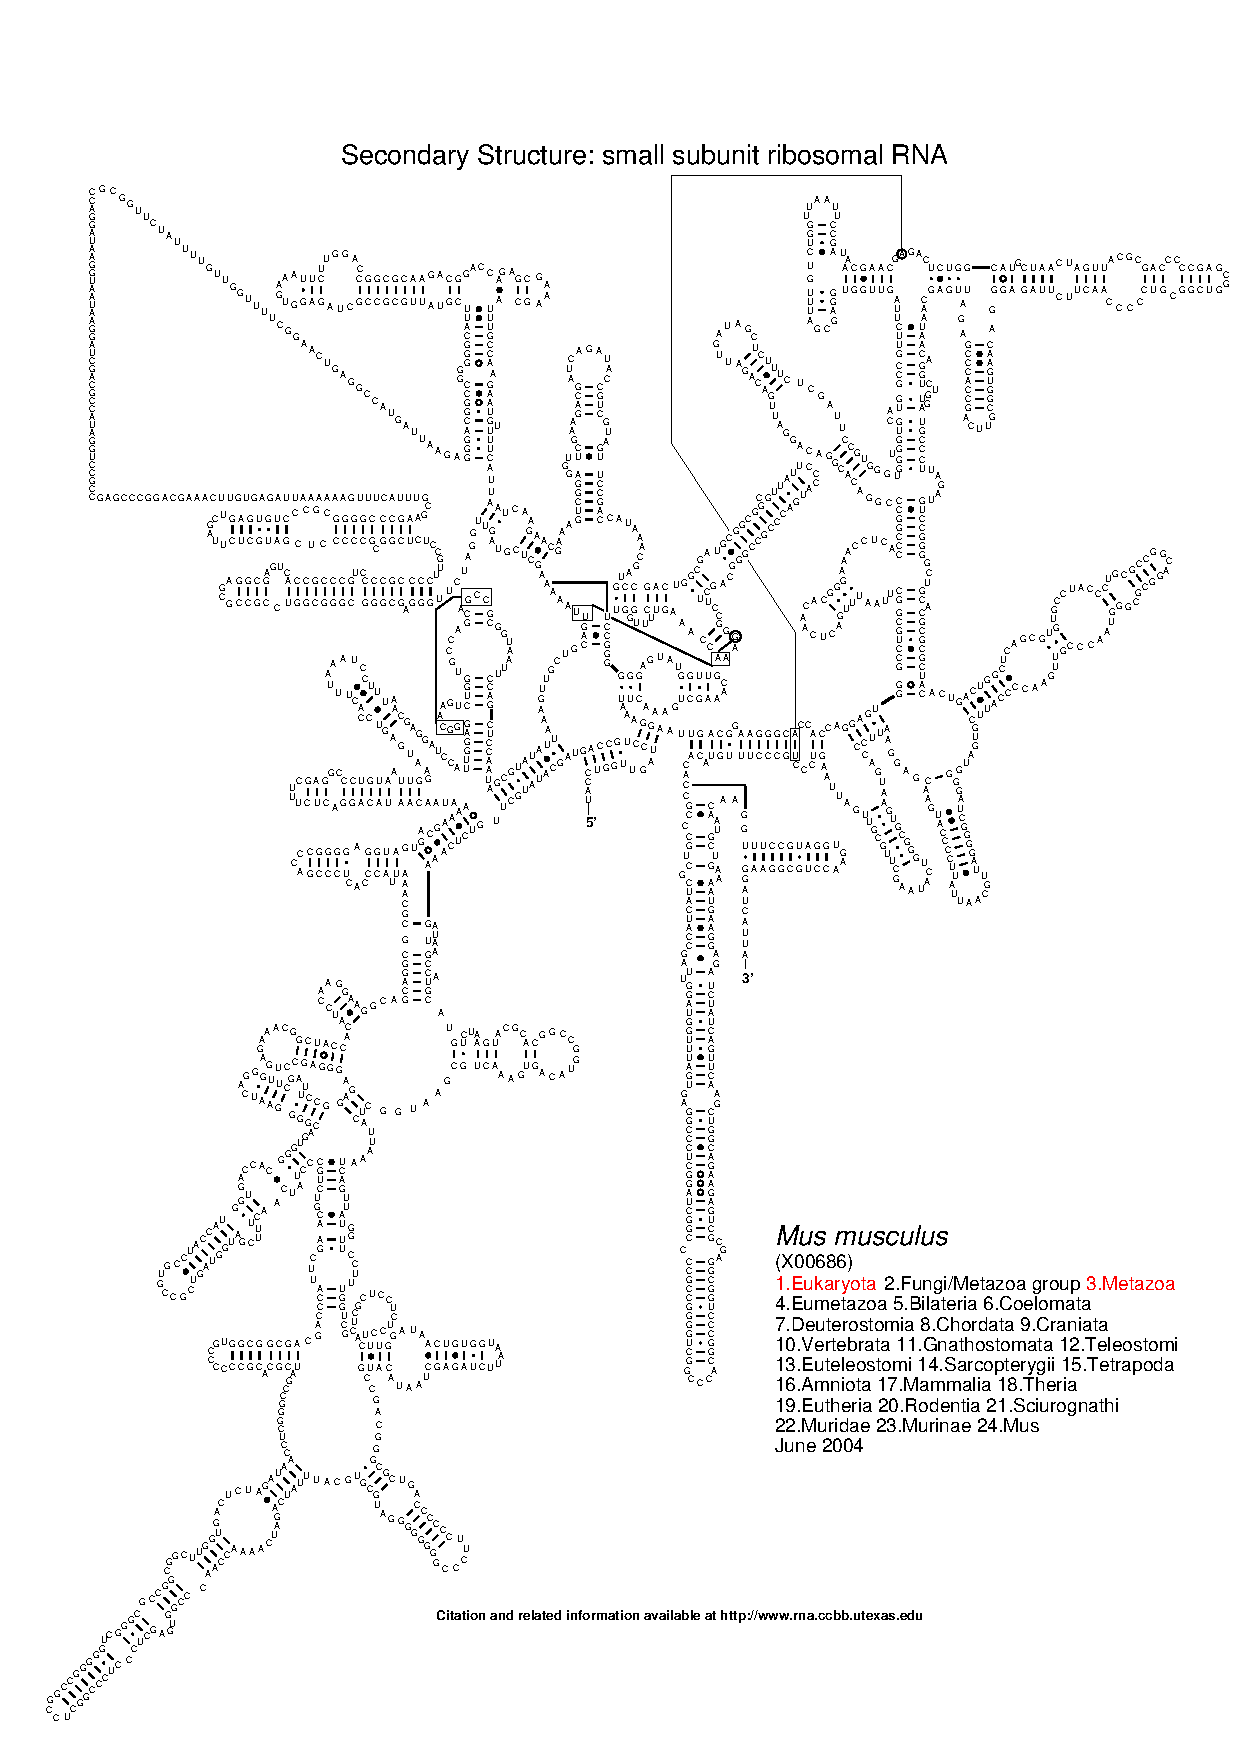
\includegraphics[width=\textwidth]{../img/mouse}}
  \caption{Príklad vstupného obrázka}
  \label{obr:mouse_ps}
\end{figure}

\section{Výstupne súbory}

Program generuje 2 druhy vystupov. Prvým je uloženie tabuľky mapovania TED algoritmu a druhým sú obrázky
vo formáte SVG a PS. \\

Označme $T1$ strom šablony a $T2$ vizualizovaný strom.

Formát mapovacieho súboru je nasledovný: \\
Prvý riadok obsahuje $DISTANCE: n$, kde $n$ je
editačná vzdialenosť medzi $T1$ a $T2$.

Ostatné riadky sú vo formáte $i$ $j$, kde $i, j \ge 0$. Inymi slovami:
\begin{itemize}
  \item 1 2 - prvý vrchol z $T1$ potrebujeme namapovať na druhý vrchol z $T2$
  \item 0 2 - do vysledného stromu vkladáme druhý vrchol z $T2$
  \item 1 0 - zo stromu $T1$ mazeme prvý vrchol
\end{itemize}

PostScript súbor je zložený z hlavičky, v ktorej sú definície kresliacich funkcií za
ktorými sú riadky kreslenia molekuly. Príklad je na obrázku \ref{obr:ps_out}.

Najprv definujeme operácie kreslenia v hlavičke súboru - $lwline$, $lwstring$ a $lwarc$ - kreslenie čiar,
textu a kružníc. Za ktorými nasleduje samotné kreslenie molekuly. \\

Podobne funguje kreslenie v SVG súbore, ktorého príklad je na obrázku \ref{obr:svg_out}.
Elementy $<text>$ vypisujú na danú pozíciu text, $<line>$
naopak kreslia čiary a $<circle>$ zase kružnice.

% TODO použivať celé príklady malej existujúcej molekuly
\begin{figure}
\begin{code}[fontsize=\scriptsize, frame=none, samepage=true]
%!
/lwline {newpath moveto lineto stroke} def
/lwstring {moveto show} def
/lwarc {newpath gsave translate scale /rad exch def /ang1 exch def /ang2 exch def 0.0 0.0
  rad ang1 ang2 arc stroke grestore} def
/Helvetica findfont 8.00 scalefont setfont
0.36 0.46 scale
219.18 1384.80 translate
0              1              0               setrgbcolor
(5')            298.311        -268.09         lwstring
0              0              0               setrgbcolor
(U)             303.3          -273            lwstring
(A)             303.3          -265            lwstring
(C)             303.3          -257            lwstring
(C)             303.501        -248.682        lwstring
305.5          -241.809       302.5          -230.191        lwline
(U)             311.246        -246.682        lwstring
  ...
showpage
\end{code}
\caption{Format vystupneho PostScript suboru}
\label{obr:ps_out}
\end{figure}

\begin{figure}
\begin{code}[fontsize=\scriptsize, frame=none, samepage=true]
<svg
  xmlns="http://www.w3.org/2000/svg"
  xmlns:xlink="http://www.w3.org/1999/xlink"
  width="1133.333333"
  height="1466.666667"
  viewBox="0 0 1139.172822px 1450.347571px"
  style="
    font-size: 8px; 
    stroke: none; 
    font-family: Helvetica; ">

  <text 
    x="517.486977"
    y="603.524781"
    style="
      stroke: rgb(0, 255, 0); ">5'</text>

  <line 
    x1="681.175823"
    y1="650.435118" 
    x2="681.175823"
    y2="662.435118"
    style="
      stroke: rgb(0, 0, 0); 
      stroke-width: 2; "/>


  <circle 
    cx="616.350806"
    cy="427.616196"
    r="6.276645"
    style="
      stroke: rgb(0, 0, 0); 
      fill: none; "/>

  ...
</svg>
\end{code}
\caption{Formát vystupného SVG súboru}
\label{obr:svg_out}
\end{figure}


\section{Rozšírenie podpory iných vstupných obrázkov}
\label{kap:rozsirenie}

Ako sme už uviedli, momentálne podporujeme iba jediný vstupný formát vstupných obrázkov.
Je ním PostScript formát používaný databázou CRW od autorov \citet{CRW}.

\begin{definice}
  Extractor bude nejaký objekt, ktorý vie zo súboru určitého typu vynať potrebné
  položky reprezentujúce RNA sekvenciu a pozíciu báz na obrázku.
\end{definice}

Pri tvorbe aplikácie sme už mysleli na budúcnosť a načítavanie súboru robíme v jednom ľahko
rozširiteľnom module. Ten sa na základe typu v parametre \param{template-tree} rozhoduje
aký extractor použiť. Predvolený a jediný implementovaný je PostScript extractor fungujúci
nad súbormi z CRW databázy.

Na implementovanie extractora potrebujeme implementovať existujúce rozhranie $extractor$,
čo znamená implementovať metódu $init$ s parametrom názvu súboru.

Jej úloha je zo súboru získať sekvenciu RNA a pozície báz.

Poslednou úlohou je pridať dvojicu $(názov\_exctractora, extractor)$ do tabuľky implementovaných
v metóde $create\_exctractors()$.

Následným volánim \param{template-tree} \param{type} $názov\_extractora$ začneme
používať nás novo implementovaný extractor.


